\documentclass[a4paper]{book}
\usepackage{a4wide}
\usepackage{makeidx}
\usepackage{graphicx}
\usepackage{multicol}
\usepackage{float}
\usepackage{listings}
\usepackage{color}
\usepackage{textcomp}
\usepackage{alltt}
\usepackage{times}
\usepackage{ifpdf}
\ifpdf
\usepackage[pdftex,
            pagebackref=true,
            colorlinks=true,
            linkcolor=blue,
            unicode
           ]{hyperref}
\else
\usepackage[ps2pdf,
            pagebackref=true,
            colorlinks=true,
            linkcolor=blue,
            unicode
           ]{hyperref}
\usepackage{pspicture}
\fi
\usepackage[utf8]{inputenc}
\usepackage{doxygen}
\lstset{language=C++,inputencoding=utf8,basicstyle=\footnotesize,breaklines=true,breakatwhitespace=true,tabsize=4,numbers=left }
\makeindex
\setcounter{tocdepth}{3}
\renewcommand{\footrulewidth}{0.4pt}
\begin{document}
\hypersetup{pageanchor=false}
\begin{titlepage}
\vspace*{7cm}
\begin{center}
{\Large oceanmodeling }\\
\vspace*{1cm}
{\large Generated by Doxygen 1.6.3}\\
\vspace*{0.5cm}
{\small Thu Apr 29 21:45:42 2010}\\
\end{center}
\end{titlepage}
\clearemptydoublepage
\pagenumbering{roman}
\tableofcontents
\clearemptydoublepage
\pagenumbering{arabic}
\hypersetup{pageanchor=true}
\chapter{Class Index}
\section{Class Hierarchy}
This inheritance list is sorted roughly, but not completely, alphabetically:\begin{DoxyCompactList}
\item \contentsline{section}{Object}{\pageref{classObject}}{}
\begin{DoxyCompactList}
\item \contentsline{section}{Hunter}{\pageref{classHunter}}{}
\item \contentsline{section}{Obstacle}{\pageref{classObstacle}}{}
\item \contentsline{section}{Prey}{\pageref{classPrey}}{}
\end{DoxyCompactList}
\item \contentsline{section}{Singleton$<$ T $>$}{\pageref{classSingleton}}{}
\item \contentsline{section}{Singleton$<$ Ocean $>$}{\pageref{classSingleton}}{}
\begin{DoxyCompactList}
\item \contentsline{section}{Ocean}{\pageref{classOcean}}{}
\end{DoxyCompactList}
\end{DoxyCompactList}

\chapter{Class Index}
\section{Class List}
Here are the classes, structs, unions and interfaces with brief descriptions:\begin{DoxyCompactList}
\item\contentsline{section}{\hyperlink{classHunter}{Hunter} }{\pageref{classHunter}}{}
\item\contentsline{section}{\hyperlink{classObject}{Object} }{\pageref{classObject}}{}
\item\contentsline{section}{\hyperlink{classObstacle}{Obstacle} }{\pageref{classObstacle}}{}
\item\contentsline{section}{\hyperlink{classOcean}{Ocean} }{\pageref{classOcean}}{}
\item\contentsline{section}{\hyperlink{classPrey}{Prey} }{\pageref{classPrey}}{}
\item\contentsline{section}{\hyperlink{classSingleton}{Singleton$<$ T $>$} }{\pageref{classSingleton}}{}
\end{DoxyCompactList}

\chapter{Class Documentation}
\hypertarget{classHunter}{
\section{Hunter Class Reference}
\label{classHunter}\index{Hunter@{Hunter}}
}
Inheritance diagram for Hunter:\begin{figure}[H]
\begin{center}
\leavevmode
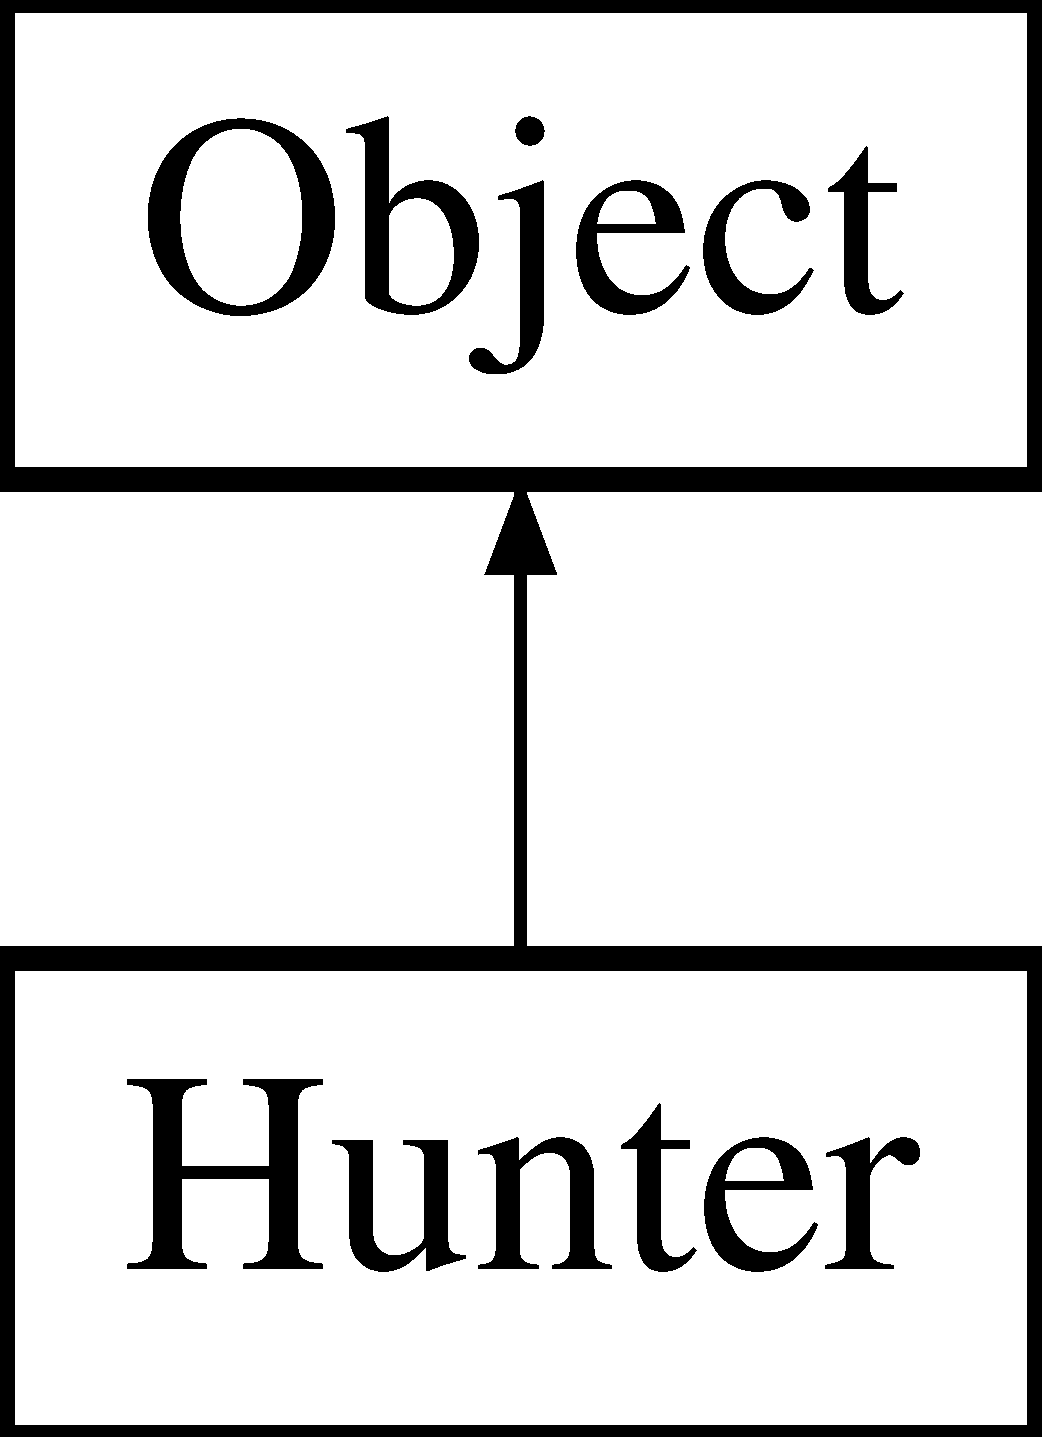
\includegraphics[height=2cm]{classHunter}
\end{center}
\end{figure}
\subsection*{Public Member Functions}
\begin{DoxyCompactItemize}
\item 
virtual void \hyperlink{classHunter_ac8bed4eeb2bfebcf7df72ba7359ac204}{Act} ()
\item 
virtual bool \hyperlink{classHunter_aad1bd13407503496a74ae1a6c689e64f}{Interact} (\hyperlink{classObject}{Object} $\ast$obj)
\item 
virtual bool \hyperlink{classHunter_aac1480382681187d650a9122dee9971c}{Dispatch} (\hyperlink{classPrey}{Prey} \&p)
\item 
virtual bool \hyperlink{classHunter_aa73667bb3b20a06d8c398eb2760e2902}{Dispatch} (\hyperlink{classHunter}{Hunter} \&h)
\item 
virtual void \hyperlink{classHunter_a9b193792622fd203df15bf755753e9bd}{PrintSelf} () const 
\end{DoxyCompactItemize}
\subsection*{Protected Member Functions}
\begin{DoxyCompactItemize}
\item 
\hypertarget{classHunter_a24cf0cbb9ca4df6886bcdff91c2aa9a2}{
{\bfseries Hunter} (int x=0, int y=0, int time\_\-to\_\-reproduce=DEFAULT\_\-TIME\_\-TO\_\-REPRODUCE, int time\_\-to\_\-die=DEFAULT\_\-TIME\_\-TO\_\-DIE)}
\label{classHunter_a24cf0cbb9ca4df6886bcdff91c2aa9a2}

\end{DoxyCompactItemize}


\subsection{Member Function Documentation}
\hypertarget{classHunter_ac8bed4eeb2bfebcf7df72ba7359ac204}{
\index{Hunter@{Hunter}!Act@{Act}}
\index{Act@{Act}!Hunter@{Hunter}}
\subsubsection[{Act}]{\setlength{\rightskip}{0pt plus 5cm}void Hunter::Act ()\hspace{0.3cm}{\ttfamily  \mbox{[}virtual\mbox{]}}}}
\label{classHunter_ac8bed4eeb2bfebcf7df72ba7359ac204}
Perform some action (die / reproduce itself / move / eat somebody) 

Implements \hyperlink{classObject_a683b351ee47dc69c4117cb9017c467d6}{Object}.

\hypertarget{classHunter_aa73667bb3b20a06d8c398eb2760e2902}{
\index{Hunter@{Hunter}!Dispatch@{Dispatch}}
\index{Dispatch@{Dispatch}!Hunter@{Hunter}}
\subsubsection[{Dispatch}]{\setlength{\rightskip}{0pt plus 5cm}virtual bool Hunter::Dispatch ({\bf Hunter} \& {\em h})\hspace{0.3cm}{\ttfamily  \mbox{[}virtual\mbox{]}}}}
\label{classHunter_aa73667bb3b20a06d8c398eb2760e2902}
Utility function needed for multiple dispatch. Return true if h is happy. 

Implements \hyperlink{classObject_a0d0e1f0456837f6736913b1ba374f11d}{Object}.

\hypertarget{classHunter_aac1480382681187d650a9122dee9971c}{
\index{Hunter@{Hunter}!Dispatch@{Dispatch}}
\index{Dispatch@{Dispatch}!Hunter@{Hunter}}
\subsubsection[{Dispatch}]{\setlength{\rightskip}{0pt plus 5cm}virtual bool Hunter::Dispatch ({\bf Prey} \& {\em p})\hspace{0.3cm}{\ttfamily  \mbox{[}virtual\mbox{]}}}}
\label{classHunter_aac1480382681187d650a9122dee9971c}
Utility function needed for multiple dispatch. Return true if p is happy. 

Implements \hyperlink{classObject_a70097e3ad4433aec0dd0b938fcedfeca}{Object}.

\hypertarget{classHunter_aad1bd13407503496a74ae1a6c689e64f}{
\index{Hunter@{Hunter}!Interact@{Interact}}
\index{Interact@{Interact}!Hunter@{Hunter}}
\subsubsection[{Interact}]{\setlength{\rightskip}{0pt plus 5cm}virtual bool Hunter::Interact ({\bf Object} $\ast$ {\em obj})\hspace{0.3cm}{\ttfamily  \mbox{[}inline, virtual\mbox{]}}}}
\label{classHunter_aad1bd13407503496a74ae1a6c689e64f}
Interaction of 2 objects. Multiple dispatch idiom (pattern visitor). Return true if this \hyperlink{classObject}{Object} is happpy after interacting with obj (e.g. hunter eats prey). 

Implements \hyperlink{classObject_a27d03e80827229de2ce885a0bc1c83c0}{Object}.

\hypertarget{classHunter_a9b193792622fd203df15bf755753e9bd}{
\index{Hunter@{Hunter}!PrintSelf@{PrintSelf}}
\index{PrintSelf@{PrintSelf}!Hunter@{Hunter}}
\subsubsection[{PrintSelf}]{\setlength{\rightskip}{0pt plus 5cm}virtual void Hunter::PrintSelf () const\hspace{0.3cm}{\ttfamily  \mbox{[}inline, virtual\mbox{]}}}}
\label{classHunter_a9b193792622fd203df15bf755753e9bd}
Print special symbol wich helps to visualize this object 

Implements \hyperlink{classObject_a2c63e79dfa8626451b4a04b0b72294eb}{Object}.



The documentation for this class was generated from the following files:\begin{DoxyCompactItemize}
\item 
object.h\item 
object.cpp\end{DoxyCompactItemize}

\hypertarget{classObject}{
\section{Object Class Reference}
\label{classObject}\index{Object@{Object}}
}
Inheritance diagram for Object:\begin{figure}[H]
\begin{center}
\leavevmode
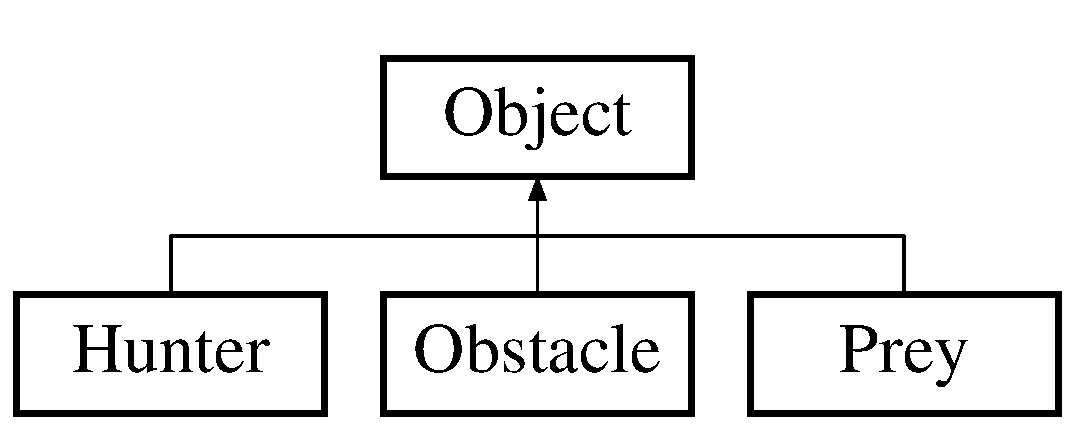
\includegraphics[height=2cm]{classObject}
\end{center}
\end{figure}
\subsection*{Public Member Functions}
\begin{DoxyCompactItemize}
\item 
virtual void \hyperlink{classObject_a683b351ee47dc69c4117cb9017c467d6}{Act} ()=0
\item 
virtual bool \hyperlink{classObject_a27d03e80827229de2ce885a0bc1c83c0}{Interact} (\hyperlink{classObject}{Object} $\ast$obj)=0
\item 
virtual bool \hyperlink{classObject_a70097e3ad4433aec0dd0b938fcedfeca}{Dispatch} (\hyperlink{classPrey}{Prey} \&p)=0
\item 
virtual bool \hyperlink{classObject_a0d0e1f0456837f6736913b1ba374f11d}{Dispatch} (\hyperlink{classHunter}{Hunter} \&h)=0
\item 
virtual void \hyperlink{classObject_a2c63e79dfa8626451b4a04b0b72294eb}{PrintSelf} () const =0
\item 
\hypertarget{classObject_acff116bb4de4bb36b38d0469defed939}{
std::pair$<$ int, int $>$ {\bfseries GetCoords} () const }
\label{classObject_acff116bb4de4bb36b38d0469defed939}

\end{DoxyCompactItemize}
\subsection*{Protected Member Functions}
\begin{DoxyCompactItemize}
\item 
\hypertarget{classObject_ad2977e29718433084247cb65894c93af}{
{\bfseries Object} (int x=0, int y=0)}
\label{classObject_ad2977e29718433084247cb65894c93af}

\item 
\hypertarget{classObject_af3b5cd7a9a24ddde484344200cf83281}{
{\bfseries Object} (const \hyperlink{classObject}{Object} \&)}
\label{classObject_af3b5cd7a9a24ddde484344200cf83281}

\item 
\hypertarget{classObject_aef3f27c97a56ab9096bc2cbc6c850bc7}{
\hyperlink{classObject}{Object} \& {\bfseries operator=} (const \hyperlink{classObject}{Object} \&)}
\label{classObject_aef3f27c97a56ab9096bc2cbc6c850bc7}

\end{DoxyCompactItemize}
\subsection*{Protected Attributes}
\begin{DoxyCompactItemize}
\item 
\hypertarget{classObject_ad0753c1468d66d4d88098f06ae2a29bb}{
int {\bfseries x\_\-}}
\label{classObject_ad0753c1468d66d4d88098f06ae2a29bb}

\item 
\hypertarget{classObject_a5fabb6445aafed3402a9431db73a8eb0}{
int {\bfseries y\_\-}}
\label{classObject_a5fabb6445aafed3402a9431db73a8eb0}

\end{DoxyCompactItemize}
\subsection*{Friends}
\begin{DoxyCompactItemize}
\item 
\hypertarget{classObject_afe3874c2dc8ab0fb894a9f3c80bfa1ad}{
class \hyperlink{classObject_afe3874c2dc8ab0fb894a9f3c80bfa1ad}{Ocean}}
\label{classObject_afe3874c2dc8ab0fb894a9f3c80bfa1ad}

\end{DoxyCompactItemize}


\subsection{Member Function Documentation}
\hypertarget{classObject_a683b351ee47dc69c4117cb9017c467d6}{
\index{Object@{Object}!Act@{Act}}
\index{Act@{Act}!Object@{Object}}
\subsubsection[{Act}]{\setlength{\rightskip}{0pt plus 5cm}virtual void Object::Act ()\hspace{0.3cm}{\ttfamily  \mbox{[}pure virtual\mbox{]}}}}
\label{classObject_a683b351ee47dc69c4117cb9017c467d6}
Perform some action (die / reproduce itself / move / eat somebody) 

Implemented in \hyperlink{classPrey_a940c0a8879376b15dedb7debf9b8f1c8}{Prey}, \hyperlink{classHunter_ac8bed4eeb2bfebcf7df72ba7359ac204}{Hunter}, and \hyperlink{classObstacle_a4e1f98a918838ca96638e7536e3748cb}{Obstacle}.

\hypertarget{classObject_a0d0e1f0456837f6736913b1ba374f11d}{
\index{Object@{Object}!Dispatch@{Dispatch}}
\index{Dispatch@{Dispatch}!Object@{Object}}
\subsubsection[{Dispatch}]{\setlength{\rightskip}{0pt plus 5cm}virtual bool Object::Dispatch ({\bf Hunter} \& {\em h})\hspace{0.3cm}{\ttfamily  \mbox{[}pure virtual\mbox{]}}}}
\label{classObject_a0d0e1f0456837f6736913b1ba374f11d}
Utility function needed for multiple dispatch. Return true if h is happy. 

Implemented in \hyperlink{classPrey_ac6b00aecc20017e58cabef00be961c6f}{Prey}, \hyperlink{classHunter_aa73667bb3b20a06d8c398eb2760e2902}{Hunter}, and \hyperlink{classObstacle_a8428a9d636c30b7c06d31066ad0dc412}{Obstacle}.

\hypertarget{classObject_a70097e3ad4433aec0dd0b938fcedfeca}{
\index{Object@{Object}!Dispatch@{Dispatch}}
\index{Dispatch@{Dispatch}!Object@{Object}}
\subsubsection[{Dispatch}]{\setlength{\rightskip}{0pt plus 5cm}virtual bool Object::Dispatch ({\bf Prey} \& {\em p})\hspace{0.3cm}{\ttfamily  \mbox{[}pure virtual\mbox{]}}}}
\label{classObject_a70097e3ad4433aec0dd0b938fcedfeca}
Utility function needed for multiple dispatch. Return true if p is happy. 

Implemented in \hyperlink{classPrey_af37fdbe20f8868903d1ffdf4fb303946}{Prey}, \hyperlink{classHunter_aac1480382681187d650a9122dee9971c}{Hunter}, and \hyperlink{classObstacle_a930bb5cb375a6554ecc76f98a8ecaf0d}{Obstacle}.

\hypertarget{classObject_a27d03e80827229de2ce885a0bc1c83c0}{
\index{Object@{Object}!Interact@{Interact}}
\index{Interact@{Interact}!Object@{Object}}
\subsubsection[{Interact}]{\setlength{\rightskip}{0pt plus 5cm}virtual bool Object::Interact ({\bf Object} $\ast$ {\em obj})\hspace{0.3cm}{\ttfamily  \mbox{[}pure virtual\mbox{]}}}}
\label{classObject_a27d03e80827229de2ce885a0bc1c83c0}
Interaction of 2 objects. Multiple dispatch idiom (pattern visitor). Return true if this \hyperlink{classObject}{Object} is happpy after interacting with obj (e.g. hunter eats prey). 

Implemented in \hyperlink{classPrey_a3f46445d442e33d47edcc94bf5f537b4}{Prey}, \hyperlink{classHunter_aad1bd13407503496a74ae1a6c689e64f}{Hunter}, and \hyperlink{classObstacle_a53bec243dc8a00f23ec61c915aef4c3e}{Obstacle}.

\hypertarget{classObject_a2c63e79dfa8626451b4a04b0b72294eb}{
\index{Object@{Object}!PrintSelf@{PrintSelf}}
\index{PrintSelf@{PrintSelf}!Object@{Object}}
\subsubsection[{PrintSelf}]{\setlength{\rightskip}{0pt plus 5cm}virtual void Object::PrintSelf () const\hspace{0.3cm}{\ttfamily  \mbox{[}pure virtual\mbox{]}}}}
\label{classObject_a2c63e79dfa8626451b4a04b0b72294eb}
Print special symbol wich helps to visualize this object 

Implemented in \hyperlink{classPrey_a46d5447bf01e734154f8d3f2f27c8fcd}{Prey}, \hyperlink{classHunter_a9b193792622fd203df15bf755753e9bd}{Hunter}, and \hyperlink{classObstacle_ad4355e9d1db002f6db2ca15ae5605d05}{Obstacle}.



The documentation for this class was generated from the following file:\begin{DoxyCompactItemize}
\item 
object.h\end{DoxyCompactItemize}

\hypertarget{classObstacle}{
\section{Obstacle Class Reference}
\label{classObstacle}\index{Obstacle@{Obstacle}}
}
Inheritance diagram for Obstacle:\begin{figure}[H]
\begin{center}
\leavevmode
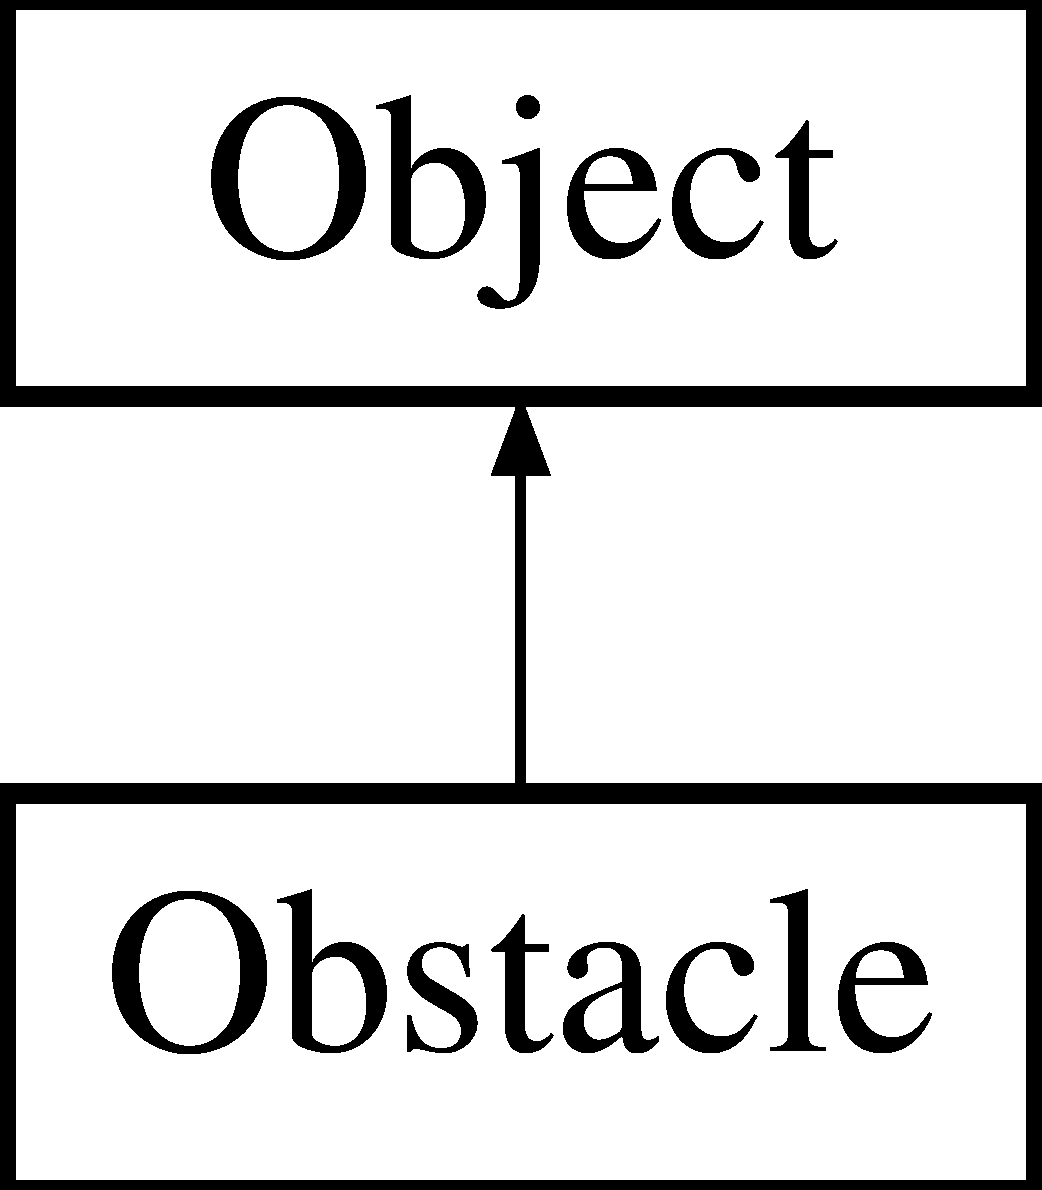
\includegraphics[height=2cm]{classObstacle}
\end{center}
\end{figure}
\subsection*{Public Member Functions}
\begin{DoxyCompactItemize}
\item 
virtual void \hyperlink{classObstacle_a4e1f98a918838ca96638e7536e3748cb}{Act} ()
\item 
virtual bool \hyperlink{classObstacle_a53bec243dc8a00f23ec61c915aef4c3e}{Interact} (\hyperlink{classObject}{Object} $\ast$)
\item 
virtual bool \hyperlink{classObstacle_a68eae0dce57aa9f5c044d4223211bfab}{Dispatch} (\hyperlink{classPrey}{Prey} \&)
\item 
virtual bool \hyperlink{classObstacle_a10634bf63cc9f11493002c7105fc7e93}{Dispatch} (\hyperlink{classHunter}{Hunter} \&)
\item 
virtual void \hyperlink{classObstacle_ad4355e9d1db002f6db2ca15ae5605d05}{PrintSelf} () const 
\end{DoxyCompactItemize}
\subsection*{Protected Member Functions}
\begin{DoxyCompactItemize}
\item 
\hypertarget{classObstacle_a57f504fff99441f6250b98ffce750a8a}{
{\bfseries Obstacle} (int x=0, int y=0)}
\label{classObstacle_a57f504fff99441f6250b98ffce750a8a}

\end{DoxyCompactItemize}
\subsection*{Friends}
\begin{DoxyCompactItemize}
\item 
\hypertarget{classObstacle_afe3874c2dc8ab0fb894a9f3c80bfa1ad}{
class \hyperlink{classObstacle_afe3874c2dc8ab0fb894a9f3c80bfa1ad}{Ocean}}
\label{classObstacle_afe3874c2dc8ab0fb894a9f3c80bfa1ad}

\end{DoxyCompactItemize}


\subsection{Member Function Documentation}
\hypertarget{classObstacle_a4e1f98a918838ca96638e7536e3748cb}{
\index{Obstacle@{Obstacle}!Act@{Act}}
\index{Act@{Act}!Obstacle@{Obstacle}}
\subsubsection[{Act}]{\setlength{\rightskip}{0pt plus 5cm}virtual void Obstacle::Act ()\hspace{0.3cm}{\ttfamily  \mbox{[}inline, virtual\mbox{]}}}}
\label{classObstacle_a4e1f98a918838ca96638e7536e3748cb}
Perform some action (die / reproduce itself / move / eat somebody) 

Implements \hyperlink{classObject_a683b351ee47dc69c4117cb9017c467d6}{Object}.

\hypertarget{classObstacle_a10634bf63cc9f11493002c7105fc7e93}{
\index{Obstacle@{Obstacle}!Dispatch@{Dispatch}}
\index{Dispatch@{Dispatch}!Obstacle@{Obstacle}}
\subsubsection[{Dispatch}]{\setlength{\rightskip}{0pt plus 5cm}bool Obstacle::Dispatch ({\bf Hunter} \& {\em h})\hspace{0.3cm}{\ttfamily  \mbox{[}virtual\mbox{]}}}}
\label{classObstacle_a10634bf63cc9f11493002c7105fc7e93}
Utility function needed for multiple dispatch. Return true if h is happy. 

Implements \hyperlink{classObject_a0d0e1f0456837f6736913b1ba374f11d}{Object}.

\hypertarget{classObstacle_a68eae0dce57aa9f5c044d4223211bfab}{
\index{Obstacle@{Obstacle}!Dispatch@{Dispatch}}
\index{Dispatch@{Dispatch}!Obstacle@{Obstacle}}
\subsubsection[{Dispatch}]{\setlength{\rightskip}{0pt plus 5cm}bool Obstacle::Dispatch ({\bf Prey} \& {\em p})\hspace{0.3cm}{\ttfamily  \mbox{[}virtual\mbox{]}}}}
\label{classObstacle_a68eae0dce57aa9f5c044d4223211bfab}
Utility function needed for multiple dispatch. Return true if p is happy. 

Implements \hyperlink{classObject_a70097e3ad4433aec0dd0b938fcedfeca}{Object}.

\hypertarget{classObstacle_a53bec243dc8a00f23ec61c915aef4c3e}{
\index{Obstacle@{Obstacle}!Interact@{Interact}}
\index{Interact@{Interact}!Obstacle@{Obstacle}}
\subsubsection[{Interact}]{\setlength{\rightskip}{0pt plus 5cm}virtual bool Obstacle::Interact ({\bf Object} $\ast$ {\em obj})\hspace{0.3cm}{\ttfamily  \mbox{[}inline, virtual\mbox{]}}}}
\label{classObstacle_a53bec243dc8a00f23ec61c915aef4c3e}
Interaction of 2 objects. Multiple dispatch idiom (pattern visitor). Return true if this \hyperlink{classObject}{Object} is happpy after interacting with obj (e.g. hunter eats prey). 

Implements \hyperlink{classObject_a27d03e80827229de2ce885a0bc1c83c0}{Object}.

\hypertarget{classObstacle_ad4355e9d1db002f6db2ca15ae5605d05}{
\index{Obstacle@{Obstacle}!PrintSelf@{PrintSelf}}
\index{PrintSelf@{PrintSelf}!Obstacle@{Obstacle}}
\subsubsection[{PrintSelf}]{\setlength{\rightskip}{0pt plus 5cm}virtual void Obstacle::PrintSelf () const\hspace{0.3cm}{\ttfamily  \mbox{[}inline, virtual\mbox{]}}}}
\label{classObstacle_ad4355e9d1db002f6db2ca15ae5605d05}
Print special symbol wich helps to visualize this object 

Implements \hyperlink{classObject_a2c63e79dfa8626451b4a04b0b72294eb}{Object}.



The documentation for this class was generated from the following files:\begin{DoxyCompactItemize}
\item 
object.h\item 
object.cpp\end{DoxyCompactItemize}

\hypertarget{classOcean}{
\section{Ocean Class Reference}
\label{classOcean}\index{Ocean@{Ocean}}
}
Inheritance diagram for Ocean:\begin{figure}[H]
\begin{center}
\leavevmode
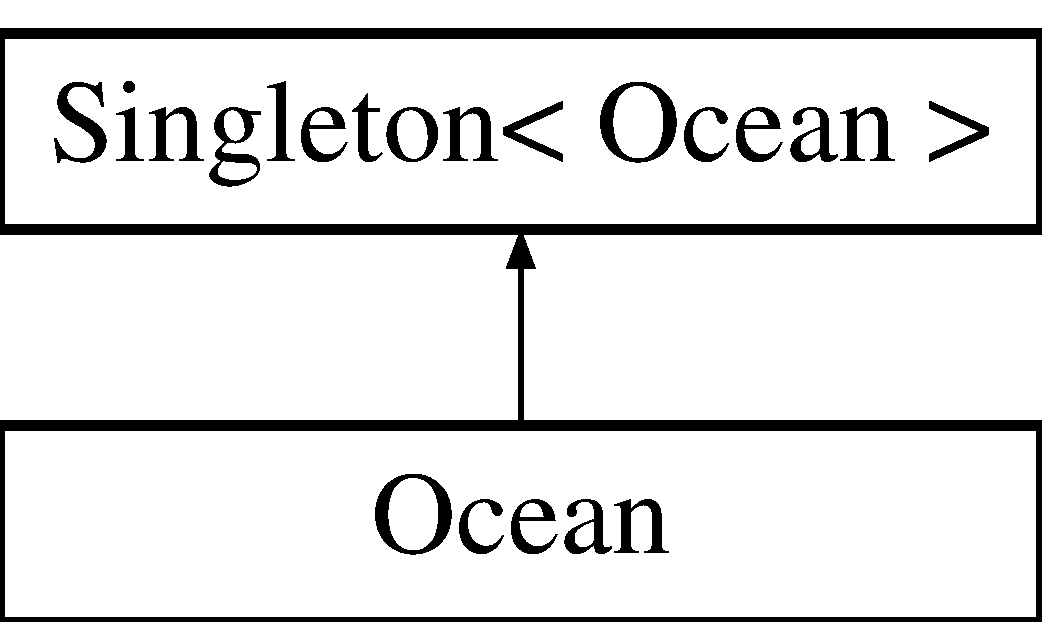
\includegraphics[height=2cm]{classOcean}
\end{center}
\end{figure}
\subsection*{Public Member Functions}
\begin{DoxyCompactItemize}
\item 
\hyperlink{classObject}{Object} $\ast$ \hyperlink{classOcean_abe1c2639f431f057509ba765682fb8cc}{GetObject} (int i, int j)
\item 
\hypertarget{classOcean_a814b481b91d9713058d481218ffb1354}{
\hyperlink{classObject}{Object} $\ast$ {\bfseries GetObject} (std::pair$<$ int, int $>$ coords)}
\label{classOcean_a814b481b91d9713058d481218ffb1354}

\item 
\hypertarget{classOcean_adfd57c71b3f5b1641cbc2c75765f9e38}{
\hyperlink{classObject}{Object} $\ast$ {\bfseries operator()} (int i, int j)}
\label{classOcean_adfd57c71b3f5b1641cbc2c75765f9e38}

\item 
void \hyperlink{classOcean_af99ba918325e6190c0185d01d53d4efb}{SetSize} (int width, int height)
\item 
void \hyperlink{classOcean_a407104f71338029cd64258afc107187a}{TicTac} ()
\item 
void \hyperlink{classOcean_ac4ebb157e229dd87113c376366f99888}{Live} ()
\item 
bool \hyperlink{classOcean_a66c18f1745faa96683ba9d42bcdec9bb}{CreateNewObject} (ObjectType t, int i, int j)
\item 
\hypertarget{classOcean_a2926e26c57d9f650c89298eadf63ccc6}{
bool {\bfseries CreateNewObject} (ObjectType t, std::pair$<$ int, int $>$ coords)}
\label{classOcean_a2926e26c57d9f650c89298eadf63ccc6}

\item 
bool \hyperlink{classOcean_a15165a09cbd8a6075d622902f562bc15}{DeleteObject} (int i, int j)
\item 
\hypertarget{classOcean_a0fbddaf476741ba579cdfbe4dde0a930}{
bool {\bfseries DeleteObject} (std::pair$<$ int, int $>$ coords)}
\label{classOcean_a0fbddaf476741ba579cdfbe4dde0a930}

\item 
bool \hyperlink{classOcean_a7b9cb70ece3c3275003ea49bdba2c2e2}{MoveObject} (\hyperlink{classObject}{Object} $\ast$obj, int i, int j)
\item 
\hypertarget{classOcean_adeab83a1c9b5baf97e963f65847b277b}{
bool {\bfseries MoveObject} (\hyperlink{classObject}{Object} $\ast$obj, std::pair$<$ int, int $>$ coords)}
\label{classOcean_adeab83a1c9b5baf97e963f65847b277b}

\item 
\hypertarget{classOcean_aae9106a2b296255a476b6dbad3ec9399}{
void {\bfseries Draw} ()}
\label{classOcean_aae9106a2b296255a476b6dbad3ec9399}

\end{DoxyCompactItemize}
\subsection*{Friends}
\begin{DoxyCompactItemize}
\item 
\hypertarget{classOcean_ae61b3a3c8247476add2d45d9cc4cb486}{
class \hyperlink{classOcean_ae61b3a3c8247476add2d45d9cc4cb486}{Singleton$<$ Ocean $>$}}
\label{classOcean_ae61b3a3c8247476add2d45d9cc4cb486}

\end{DoxyCompactItemize}


\subsection{Member Function Documentation}
\hypertarget{classOcean_a66c18f1745faa96683ba9d42bcdec9bb}{
\index{Ocean@{Ocean}!CreateNewObject@{CreateNewObject}}
\index{CreateNewObject@{CreateNewObject}!Ocean@{Ocean}}
\subsubsection[{CreateNewObject}]{\setlength{\rightskip}{0pt plus 5cm}bool Ocean::CreateNewObject (ObjectType {\em t}, \/  int {\em i}, \/  int {\em j})\hspace{0.3cm}{\ttfamily  \mbox{[}inline\mbox{]}}}}
\label{classOcean_a66c18f1745faa96683ba9d42bcdec9bb}
Create new object of type t under the coordinates (i, j). Return false if operation fails. \hypertarget{classOcean_a15165a09cbd8a6075d622902f562bc15}{
\index{Ocean@{Ocean}!DeleteObject@{DeleteObject}}
\index{DeleteObject@{DeleteObject}!Ocean@{Ocean}}
\subsubsection[{DeleteObject}]{\setlength{\rightskip}{0pt plus 5cm}bool Ocean::DeleteObject (int {\em i}, \/  int {\em j})\hspace{0.3cm}{\ttfamily  \mbox{[}inline\mbox{]}}}}
\label{classOcean_a15165a09cbd8a6075d622902f562bc15}
Delete object under the coordinates (i, j) (if any). Return false if operation fails. \hypertarget{classOcean_abe1c2639f431f057509ba765682fb8cc}{
\index{Ocean@{Ocean}!GetObject@{GetObject}}
\index{GetObject@{GetObject}!Ocean@{Ocean}}
\subsubsection[{GetObject}]{\setlength{\rightskip}{0pt plus 5cm}{\bf Object}$\ast$ Ocean::GetObject (int {\em i}, \/  int {\em j})\hspace{0.3cm}{\ttfamily  \mbox{[}inline\mbox{]}}}}
\label{classOcean_abe1c2639f431f057509ba765682fb8cc}
Return pointer to the object located by coordinates (i, j) if any or NULL pointer otherwise \hypertarget{classOcean_ac4ebb157e229dd87113c376366f99888}{
\index{Ocean@{Ocean}!Live@{Live}}
\index{Live@{Live}!Ocean@{Ocean}}
\subsubsection[{Live}]{\setlength{\rightskip}{0pt plus 5cm}void Ocean::Live ()\hspace{0.3cm}{\ttfamily  \mbox{[}inline\mbox{]}}}}
\label{classOcean_ac4ebb157e229dd87113c376366f99888}
ocean starts it's life \hypertarget{classOcean_a7b9cb70ece3c3275003ea49bdba2c2e2}{
\index{Ocean@{Ocean}!MoveObject@{MoveObject}}
\index{MoveObject@{MoveObject}!Ocean@{Ocean}}
\subsubsection[{MoveObject}]{\setlength{\rightskip}{0pt plus 5cm}bool Ocean::MoveObject ({\bf Object} $\ast$ {\em obj}, \/  int {\em i}, \/  int {\em j})\hspace{0.3cm}{\ttfamily  \mbox{[}inline\mbox{]}}}}
\label{classOcean_a7b9cb70ece3c3275003ea49bdba2c2e2}
Move object to the coordinates (i, j). Return false if operation fails. \hypertarget{classOcean_af99ba918325e6190c0185d01d53d4efb}{
\index{Ocean@{Ocean}!SetSize@{SetSize}}
\index{SetSize@{SetSize}!Ocean@{Ocean}}
\subsubsection[{SetSize}]{\setlength{\rightskip}{0pt plus 5cm}void Ocean::SetSize (int {\em width}, \/  int {\em height})\hspace{0.3cm}{\ttfamily  \mbox{[}inline\mbox{]}}}}
\label{classOcean_af99ba918325e6190c0185d01d53d4efb}
Sets size of ocean \hypertarget{classOcean_a407104f71338029cd64258afc107187a}{
\index{Ocean@{Ocean}!TicTac@{TicTac}}
\index{TicTac@{TicTac}!Ocean@{Ocean}}
\subsubsection[{TicTac}]{\setlength{\rightskip}{0pt plus 5cm}void Ocean::TicTac ()\hspace{0.3cm}{\ttfamily  \mbox{[}inline\mbox{]}}}}
\label{classOcean_a407104f71338029cd64258afc107187a}
Time is money 

The documentation for this class was generated from the following file:\begin{DoxyCompactItemize}
\item 
ocean.hpp\end{DoxyCompactItemize}

\hypertarget{classPrey}{
\section{Prey Class Reference}
\label{classPrey}\index{Prey@{Prey}}
}
Inheritance diagram for Prey:\begin{figure}[H]
\begin{center}
\leavevmode
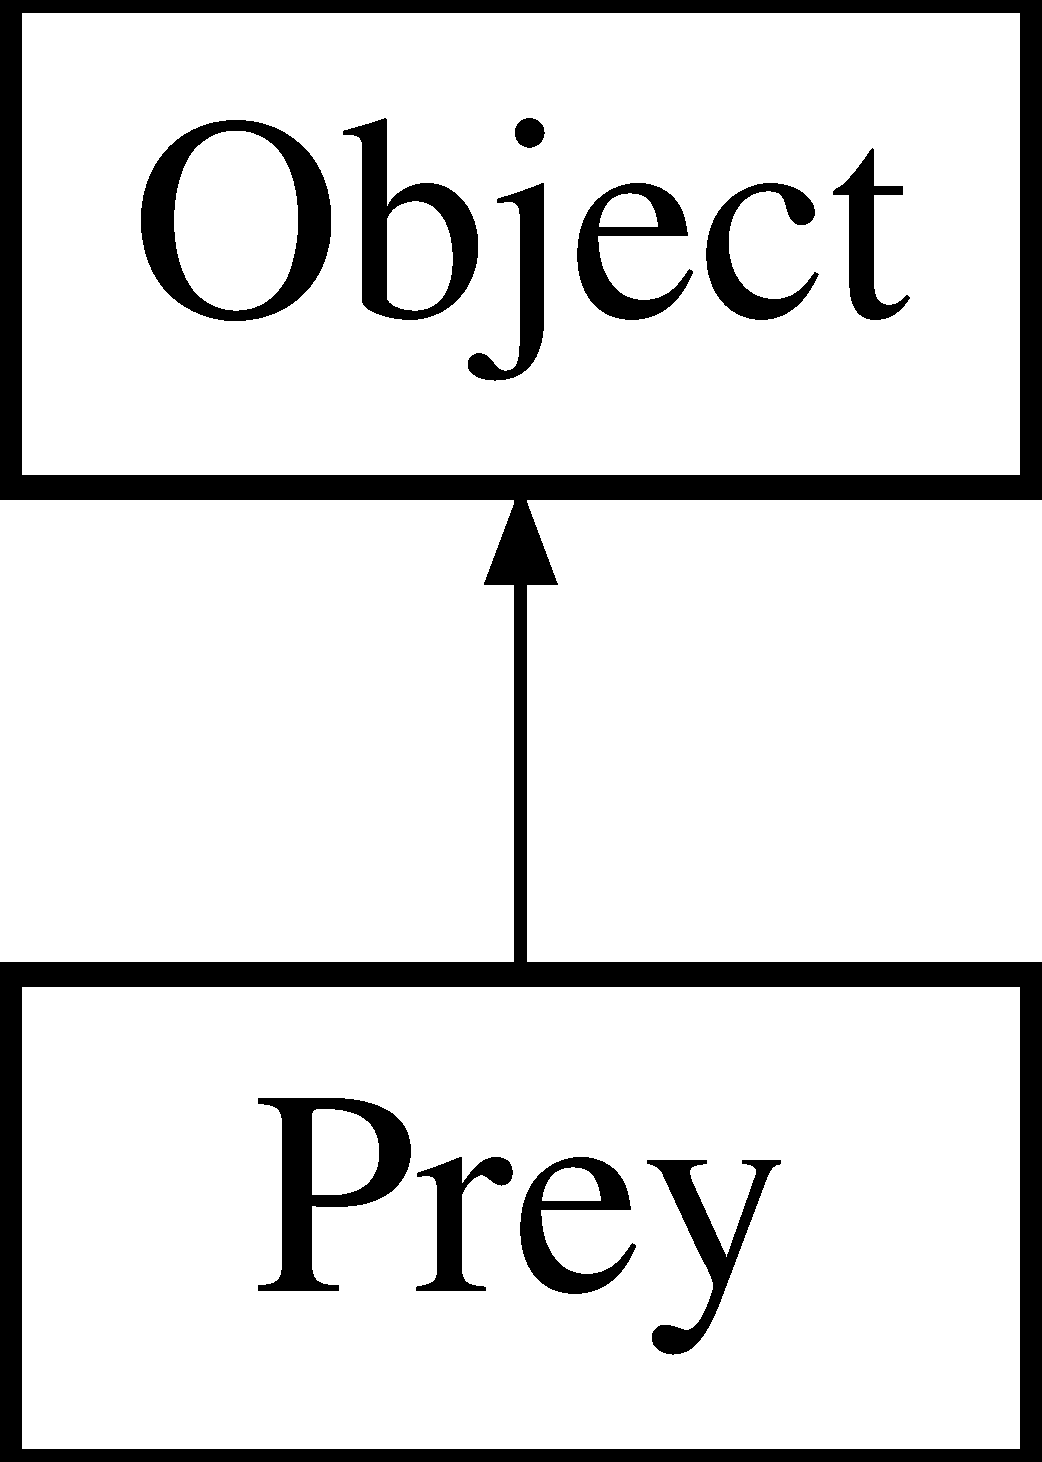
\includegraphics[height=2cm]{classPrey}
\end{center}
\end{figure}
\subsection*{Public Member Functions}
\begin{DoxyCompactItemize}
\item 
virtual void \hyperlink{classPrey_a940c0a8879376b15dedb7debf9b8f1c8}{Act} ()
\item 
virtual bool \hyperlink{classPrey_a3f46445d442e33d47edcc94bf5f537b4}{Interact} (\hyperlink{classObject}{Object} $\ast$obj)
\item 
virtual bool \hyperlink{classPrey_af37fdbe20f8868903d1ffdf4fb303946}{Dispatch} (\hyperlink{classPrey}{Prey} \&p)
\item 
virtual bool \hyperlink{classPrey_ac6b00aecc20017e58cabef00be961c6f}{Dispatch} (\hyperlink{classHunter}{Hunter} \&h)
\item 
virtual void \hyperlink{classPrey_a46d5447bf01e734154f8d3f2f27c8fcd}{PrintSelf} () const 
\end{DoxyCompactItemize}
\subsection*{Protected Member Functions}
\begin{DoxyCompactItemize}
\item 
\hypertarget{classPrey_a1e65463a2ed66b174fcd735676b0d68e}{
{\bfseries Prey} (int x=0, int y=0, int time\_\-to\_\-reproduce=DEFAULT\_\-TIME\_\-TO\_\-REPRODUCE)}
\label{classPrey_a1e65463a2ed66b174fcd735676b0d68e}

\end{DoxyCompactItemize}
\subsection*{Friends}
\begin{DoxyCompactItemize}
\item 
\hypertarget{classPrey_a0720b5f434e636e22a3ed34f847eec57}{
class \hyperlink{classPrey_a0720b5f434e636e22a3ed34f847eec57}{Object}}
\label{classPrey_a0720b5f434e636e22a3ed34f847eec57}

\end{DoxyCompactItemize}


\subsection{Member Function Documentation}
\hypertarget{classPrey_a940c0a8879376b15dedb7debf9b8f1c8}{
\index{Prey@{Prey}!Act@{Act}}
\index{Act@{Act}!Prey@{Prey}}
\subsubsection[{Act}]{\setlength{\rightskip}{0pt plus 5cm}void Prey::Act ()\hspace{0.3cm}{\ttfamily  \mbox{[}virtual\mbox{]}}}}
\label{classPrey_a940c0a8879376b15dedb7debf9b8f1c8}
Perform some action (die / reproduce itself / move / eat somebody) 

Implements \hyperlink{classObject_a683b351ee47dc69c4117cb9017c467d6}{Object}.

\hypertarget{classPrey_ac6b00aecc20017e58cabef00be961c6f}{
\index{Prey@{Prey}!Dispatch@{Dispatch}}
\index{Dispatch@{Dispatch}!Prey@{Prey}}
\subsubsection[{Dispatch}]{\setlength{\rightskip}{0pt plus 5cm}virtual bool Prey::Dispatch ({\bf Hunter} \& {\em h})\hspace{0.3cm}{\ttfamily  \mbox{[}virtual\mbox{]}}}}
\label{classPrey_ac6b00aecc20017e58cabef00be961c6f}
Utility function needed for multiple dispatch. Return true if h is happy. 

Implements \hyperlink{classObject_a0d0e1f0456837f6736913b1ba374f11d}{Object}.

\hypertarget{classPrey_af37fdbe20f8868903d1ffdf4fb303946}{
\index{Prey@{Prey}!Dispatch@{Dispatch}}
\index{Dispatch@{Dispatch}!Prey@{Prey}}
\subsubsection[{Dispatch}]{\setlength{\rightskip}{0pt plus 5cm}virtual bool Prey::Dispatch ({\bf Prey} \& {\em p})\hspace{0.3cm}{\ttfamily  \mbox{[}virtual\mbox{]}}}}
\label{classPrey_af37fdbe20f8868903d1ffdf4fb303946}
Utility function needed for multiple dispatch. Return true if p is happy. 

Implements \hyperlink{classObject_a70097e3ad4433aec0dd0b938fcedfeca}{Object}.

\hypertarget{classPrey_a3f46445d442e33d47edcc94bf5f537b4}{
\index{Prey@{Prey}!Interact@{Interact}}
\index{Interact@{Interact}!Prey@{Prey}}
\subsubsection[{Interact}]{\setlength{\rightskip}{0pt plus 5cm}virtual bool Prey::Interact ({\bf Object} $\ast$ {\em obj})\hspace{0.3cm}{\ttfamily  \mbox{[}inline, virtual\mbox{]}}}}
\label{classPrey_a3f46445d442e33d47edcc94bf5f537b4}
Interaction of 2 objects. Multiple dispatch idiom (pattern visitor). Return true if this \hyperlink{classObject}{Object} is happpy after interacting with obj (e.g. hunter eats prey). 

Implements \hyperlink{classObject_a27d03e80827229de2ce885a0bc1c83c0}{Object}.

\hypertarget{classPrey_a46d5447bf01e734154f8d3f2f27c8fcd}{
\index{Prey@{Prey}!PrintSelf@{PrintSelf}}
\index{PrintSelf@{PrintSelf}!Prey@{Prey}}
\subsubsection[{PrintSelf}]{\setlength{\rightskip}{0pt plus 5cm}virtual void Prey::PrintSelf () const\hspace{0.3cm}{\ttfamily  \mbox{[}inline, virtual\mbox{]}}}}
\label{classPrey_a46d5447bf01e734154f8d3f2f27c8fcd}
Print special symbol wich helps to visualize this object 

Implements \hyperlink{classObject_a2c63e79dfa8626451b4a04b0b72294eb}{Object}.



The documentation for this class was generated from the following files:\begin{DoxyCompactItemize}
\item 
object.h\item 
object.cpp\end{DoxyCompactItemize}

\hypertarget{classSingleton}{
\section{Singleton$<$ T $>$ Class Template Reference}
\label{classSingleton}\index{Singleton@{Singleton}}
}
\subsection*{Static Public Member Functions}
\begin{DoxyCompactItemize}
\item 
\hypertarget{classSingleton_a131e87528259529400d58b6df5d9743c}{
static T \& {\bfseries Instance} ()}
\label{classSingleton_a131e87528259529400d58b6df5d9743c}

\end{DoxyCompactItemize}
\subsection*{Protected Member Functions}
\begin{DoxyCompactItemize}
\item 
\hypertarget{classSingleton_a363d3f7d5276e6ee74966d9606df2086}{
{\bfseries Singleton} (const \hyperlink{classSingleton}{Singleton} \&)}
\label{classSingleton_a363d3f7d5276e6ee74966d9606df2086}

\item 
\hypertarget{classSingleton_a90761b9486d76162ab59c871b5cc030f}{
\hyperlink{classSingleton}{Singleton} \& {\bfseries operator=} (const \hyperlink{classSingleton}{Singleton} \&)}
\label{classSingleton_a90761b9486d76162ab59c871b5cc030f}

\end{DoxyCompactItemize}
\subsubsection*{template$<$typename T$>$ class Singleton$<$ T $>$}



The documentation for this class was generated from the following file:\begin{DoxyCompactItemize}
\item 
ocean.hpp\end{DoxyCompactItemize}

\printindex
\end{document}
